\section{Materiales y métodos}

\subsection{Diseño experimental}

El presente trabajo consistió en el estudio del efecto de campos magnéticos estáticos sobre semillas de maíz, mediante un esquema experimental que requirió la organización controlada de muestras, su disposición en un sistema de tratamiento reproducible y el registro sistemático de variables asociadas al proceso de germinación.

Con el fin de garantizar la factibilidad, reproducibilidad y organización del protocolo experimental, fue necesaria una etapa preliminar de diseño y preparación del sistema de trabajo. Esta etapa incluyó el desarrollo de dispositivos físicos para el tratamiento y manipulación de las semillas, la fabricación de piezas mediante impresión 3D, la implementación de herramientas informáticas para automatizar tareas de organización y análisis, y la construcción de un sistema estandarizado de adquisición de imágenes.

\subsection{Materiales empleados}

Para el desarrollo experimental se utilizaron semillas de maíz, estructuras de soporte y contención fabricadas mediante impresión 3D, imanes permanentes para el tratamiento magnético, y un sistema de adquisición de imágenes construido específicamente para este trabajo.

El diseño de piezas se realizó principalmente con \textit{Tinkercad}, complementado en algunos casos con \textit{build123d}, especialmente cuando se requirieron modificaciones paramétricas o ajustes sistemáticos de dimensiones. Las tareas de programación asociadas a este trabajo se realizaron utilizando \textit{Visual Studio Code} como entorno principal de desarrollo.

Para la adquisición de imágenes se construyó un \textit{photobox}, consistente en una caja con fondo negro e iluminación LED, diseñado con el objetivo de mejorar el contraste y estandarizar las condiciones de captura.

Finalmente, cabe señalar que el sistema PID utilizado en el laboratorio ya se encontraba previamente implementado en el MBLab por otros integrantes, por lo que no forma parte del desarrollo original de esta tesis.

\subsection{Caracterización de los imanes}

Con el fin de conocer el perfil espacial del campo magnético generado por los imanes utilizados en los tratamientos, se realizó una caracterización experimental del campo en función de la distancia a la cara del imán. Para ello se empleó un gaussímetro con sonda Hall, registrándose la intensidad de campo magnético (mT) sobre el eje central de la cara del imán (\textit{Centro}) y sobre sus cuatro esquinas (\textit{Esq A}, \textit{Esq B}, \textit{Esq C} y \textit{Esq D}), a una serie de distancias crecientes respecto de la superficie del imán.

La Figura~\ref{fig:ceramica_n_perfil} muestra el perfil de campo obtenido para el imán de cerámica, polo norte. Como es esperable, la intensidad de campo decae de forma pronunciada con la distancia, y las mediciones tomadas en el centro resultan sistemáticamente algo mayores que las obtenidas en las esquinas, reflejando la distribución no uniforme del campo sobre la cara del imán.

\begin{figure}[H]
    \centering
    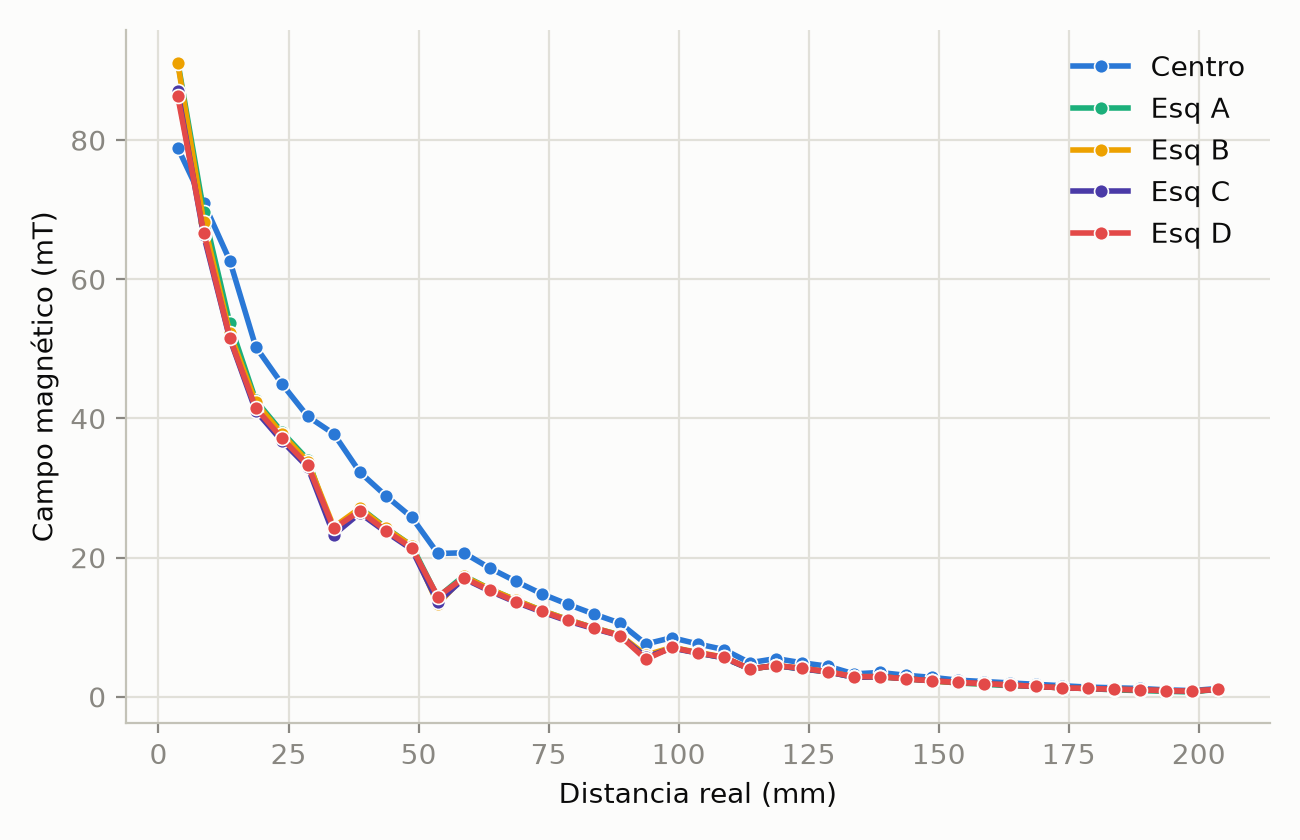
\includegraphics[width=0.85\linewidth]{datos/img/ceramica_n_perfil.png}
    \caption{Caracterización del campo magnético del imán de cerámica, polo norte, en función de la distancia a su cara. Se muestran las mediciones tomadas en el centro y en las cuatro esquinas de la cara del imán.}
    \label{fig:ceramica_n_perfil}
\end{figure}

Un comportamiento equivalente se observó para el imán de cerámica, polo sur (Figura~\ref{fig:ceramica_s_perfil}), donde nuevamente el centro presenta los valores más elevados y las cuatro esquinas se agrupan entre sí, con una caída marcada del campo dentro de los primeros 50~mm.

\begin{figure}[H]
    \centering
    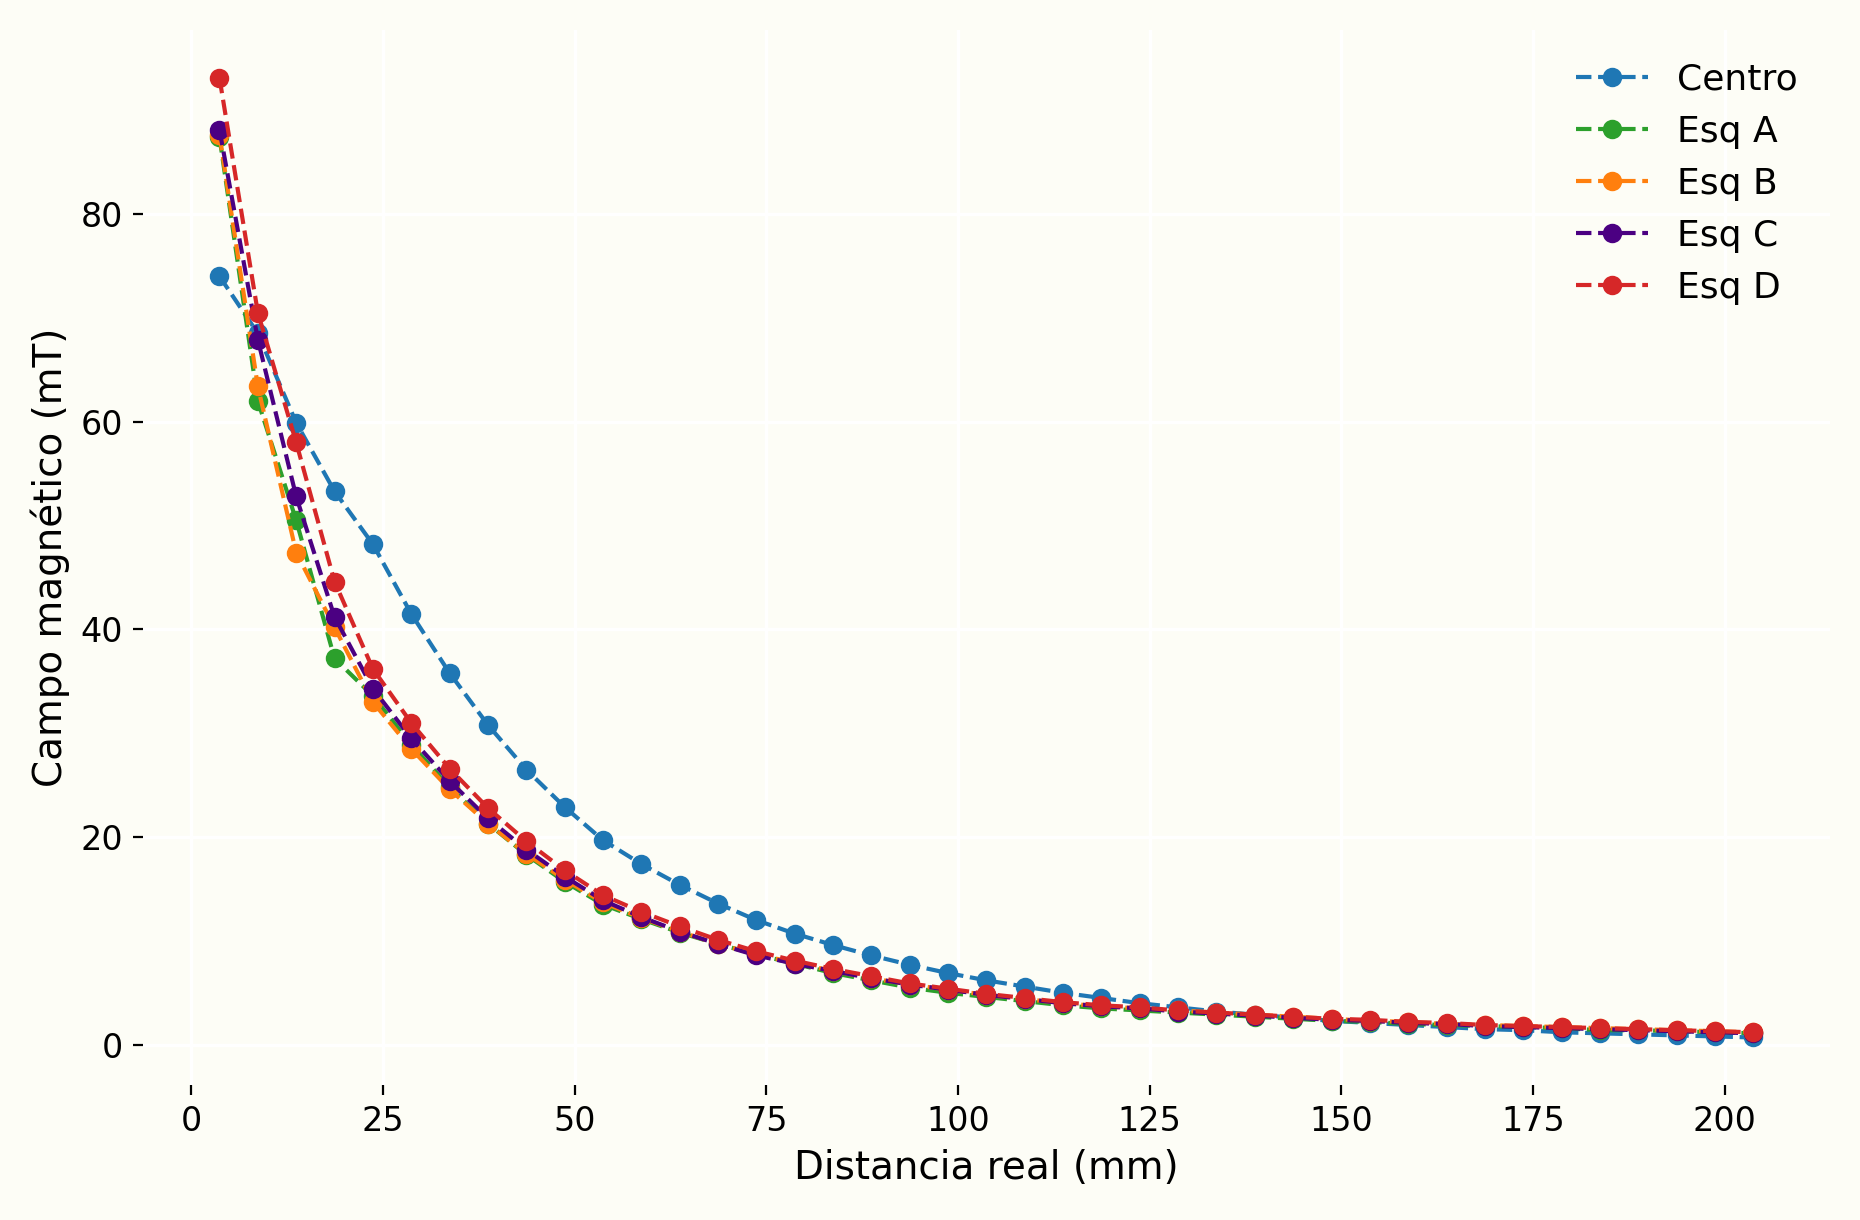
\includegraphics[width=0.85\linewidth]{datos/img/ceramica_s_perfil.png}
    \caption{Caracterización del campo magnético del imán de cerámica, polo sur, en función de la distancia a su cara. Se muestran las mediciones tomadas en el centro y en las cuatro esquinas de la cara del imán.}
    \label{fig:ceramica_s_perfil}
\end{figure}

El imán de neodimio, polo norte, presentó un campo considerablemente más intenso que los imanes de cerámica, alcanzando cerca de 295~mT en el centro a la mínima distancia medida (Figura~\ref{fig:neodimio_n_perfil}). A diferencia de los imanes de cerámica, las mediciones en las esquinas no decrecen monótonamente desde el primer punto, sino que muestran un máximo local a pocos milímetros de la cara antes de decaer, lo cual es consistente con la geometría y distribución de flujo característica de los imanes de neodimio de mayor intensidad.

\begin{figure}[H]
    \centering
    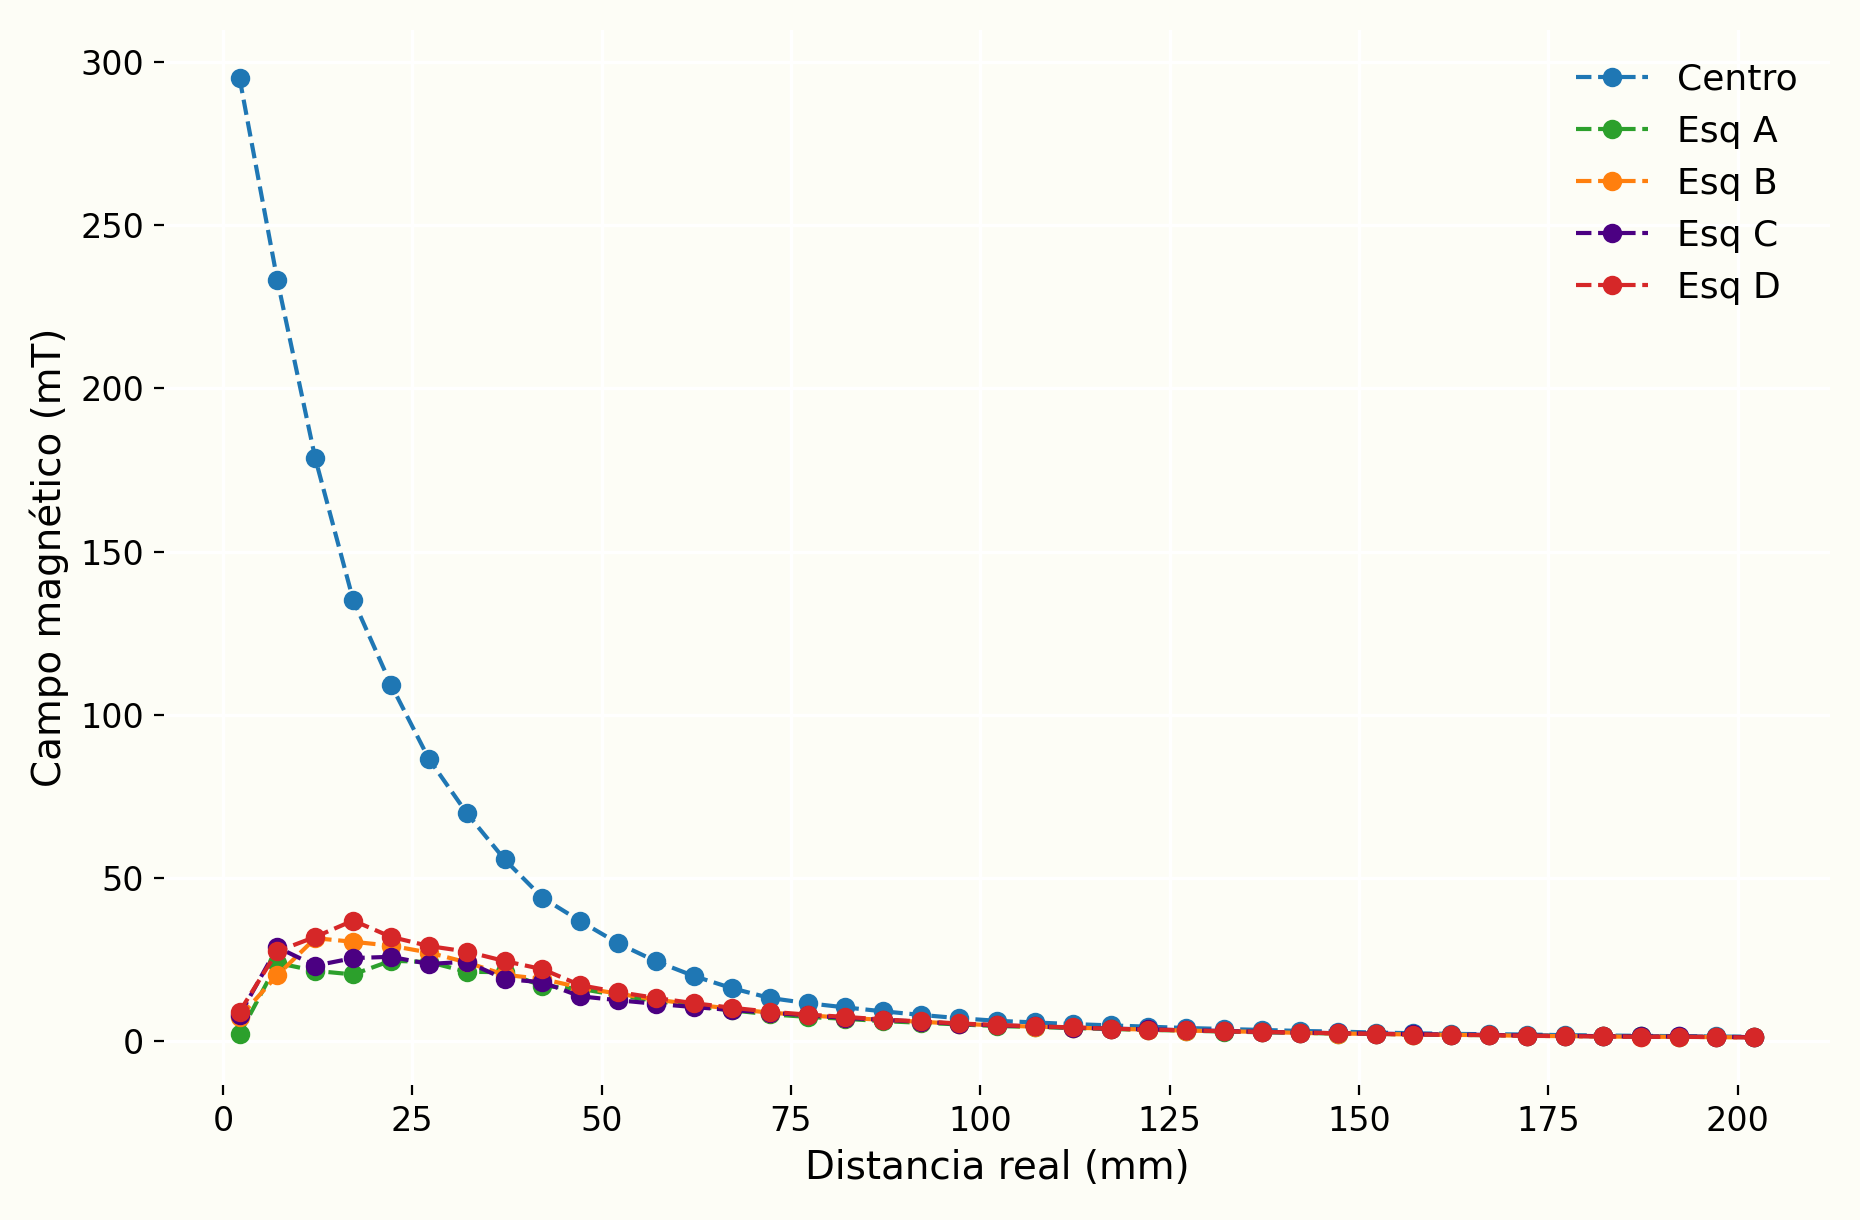
\includegraphics[width=0.85\linewidth]{datos/img/neodimio_n_perfil.png}
    \caption{Caracterización del campo magnético del imán de neodimio, polo norte, en función de la distancia a su cara. Se muestran las mediciones tomadas en el centro y en las cuatro esquinas de la cara del imán.}
    \label{fig:neodimio_n_perfil}
\end{figure}

\subsection{Montaje experimental}

\subsubsection{Diseño de la torre y semilleros}

Se diseñó una estructura experimental compuesta por una torre y un conjunto de semilleros destinada a alojar las semillas durante la etapa de exposición magnética. El objetivo principal de este sistema fue asegurar una disposición geométrica reproducible de las muestras, permitiendo ubicar las semillas en posiciones controladas dentro del montaje experimental.

Durante el diseño se buscó que las piezas cumplieran simultáneamente varios requisitos: contener adecuadamente las semillas, facilitar su manipulación antes y después de la germinación, mantener una disposición estable durante el tratamiento y resultar compatibles con fabricación mediante impresión 3D. Asimismo, se procuró que la geometría del sistema permitiera trabajar de forma ordenada con distintos niveles o posiciones experimentales.

El modelado de la geometría se realizó principalmente en \textit{Tinkercad}, herramienta utilizada para desarrollar la estructura general de la torre y los semilleros. En algunos casos particulares, especialmente cuando se requirieron modificaciones paramétricas o ajustes más sistemáticos, se empleó también \textit{build123d}.

A lo largo del desarrollo fue necesario realizar ajustes sucesivos sobre las dimensiones y el diseño de las piezas, con el fin de mejorar aspectos de calce, estabilidad mecánica y facilidad de uso. Una vez obtenidas versiones satisfactorias, las piezas fueron fabricadas mediante impresión 3D e incorporadas al sistema experimental.

La Figura~\ref{fig:torre_semilleros} muestra, lado a lado, el diseño digital y la pieza ya impresa. Los archivos de diseño y desarrollo asociados se encuentran documentados en el repositorio del proyecto.

\begin{figure}[H]
    \centering
    \begin{subfigure}[b]{0.45\linewidth}
        \centering
        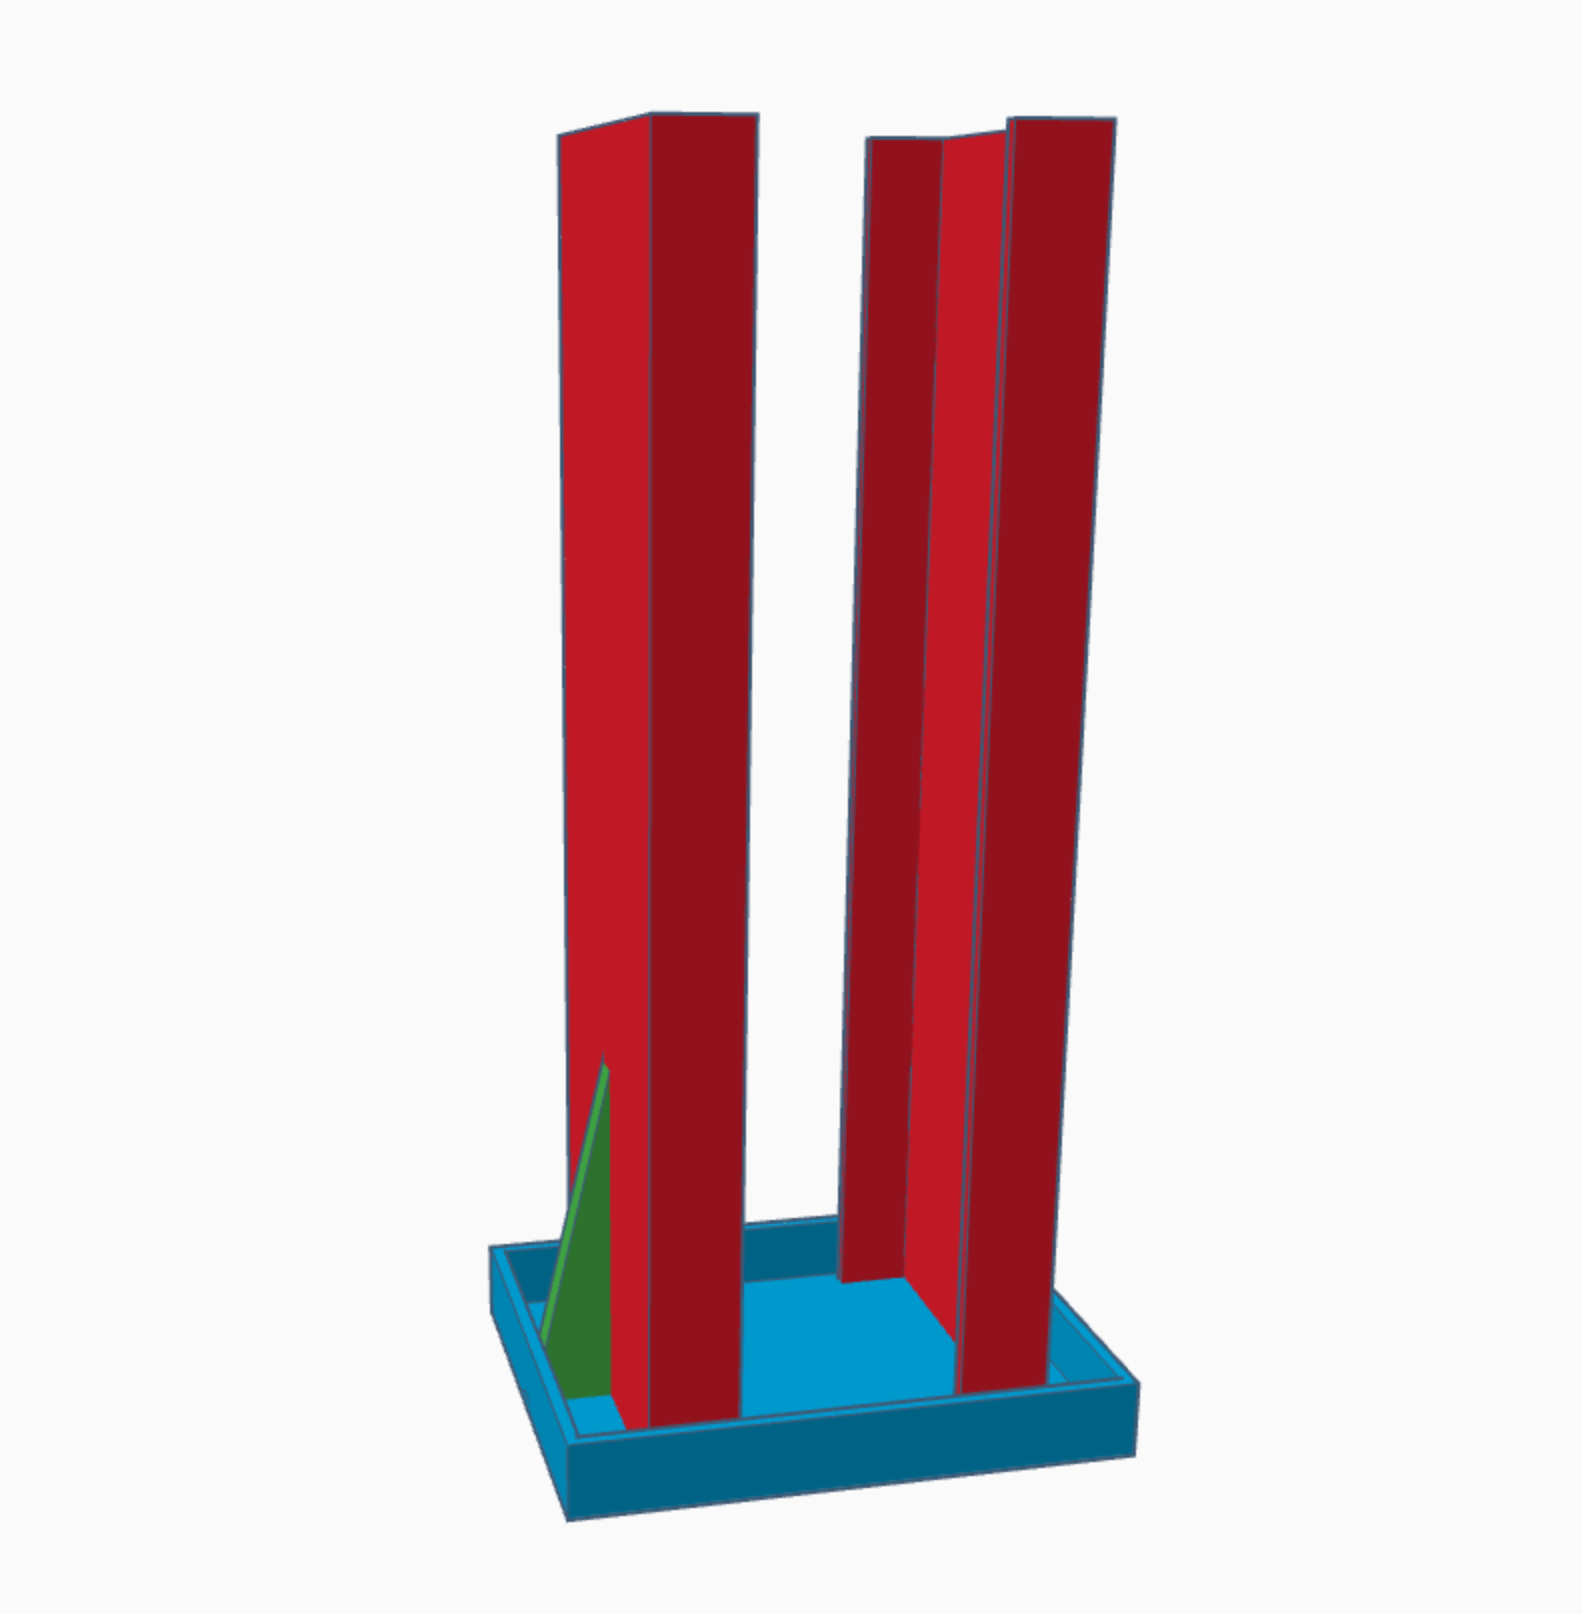
\includegraphics[width=\linewidth]{secciones//images/torre3D.png}
        \caption{Diseño 3D}
    \end{subfigure}
    \hfill
    \begin{subfigure}[b]{0.28\linewidth}
        \centering
        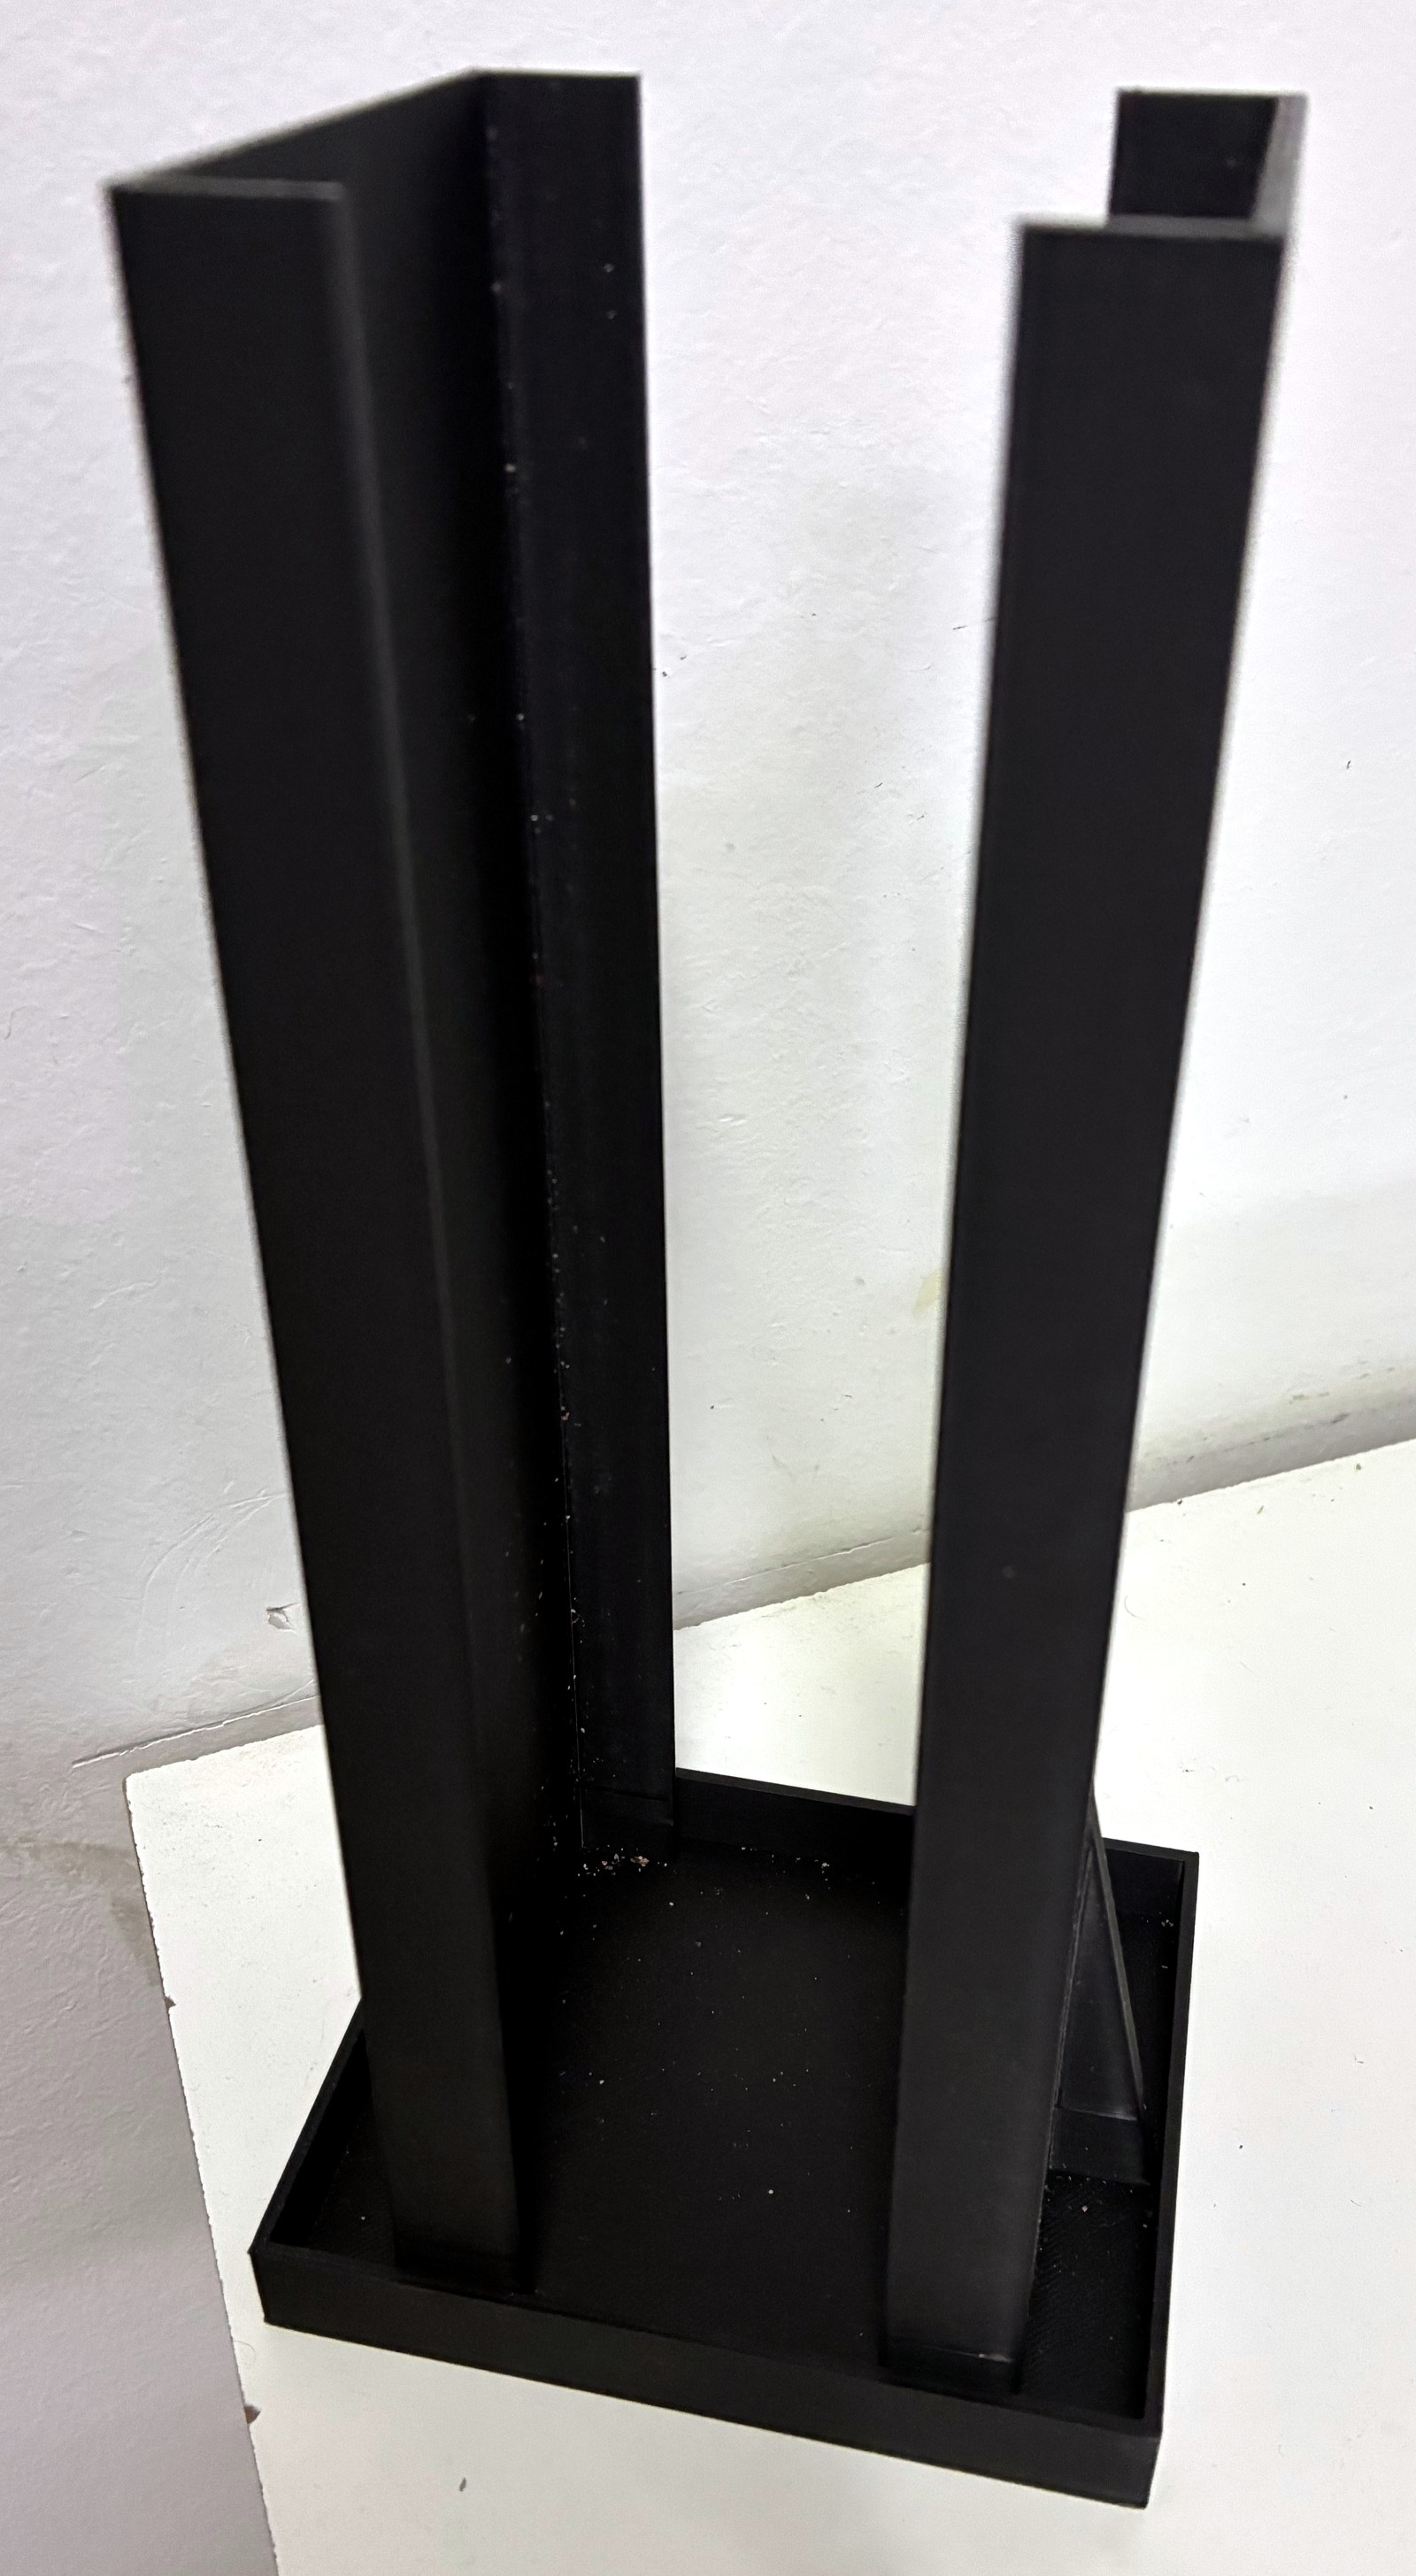
\includegraphics[width=\linewidth]{datos/img/torre_foto.jpg}
        \caption{Pieza impresa}
    \end{subfigure}
    \caption{Torre utilizada para alojar los cajones durante el tratamiento magnético: diseño realizado en \textit{Tinkercad} y pieza final fabricada mediante impresión 3D.}
    \label{fig:torre_semilleros}
\end{figure}

\subsubsection{Cajón portasemillas}

Como parte de este sistema, se diseñó un cajón destinado a contener las semillas durante el tratamiento. En su diseño se buscó que permitiera una disposición ordenada de las muestras, facilitara su manipulación y resultara compatible con el resto de la estructura experimental. Asimismo, se procuró que sus dimensiones fueran adecuadas para el alojamiento de las semillas y para su fabricación mediante impresión 3D.

El modelado de estas piezas se realizó principalmente en \textit{Tinkercad}, complementado en algunos casos con \textit{build123d} para ajustes paramétricos. Las versiones finales fueron fabricadas mediante impresión 3D. En la Figura~\ref{fig:cajon_semillas} se muestra, lado a lado, el diseño y la pieza física utilizada.

\begin{figure}[H]
    \centering
    \begin{subfigure}[b]{0.45\linewidth}
        \centering
        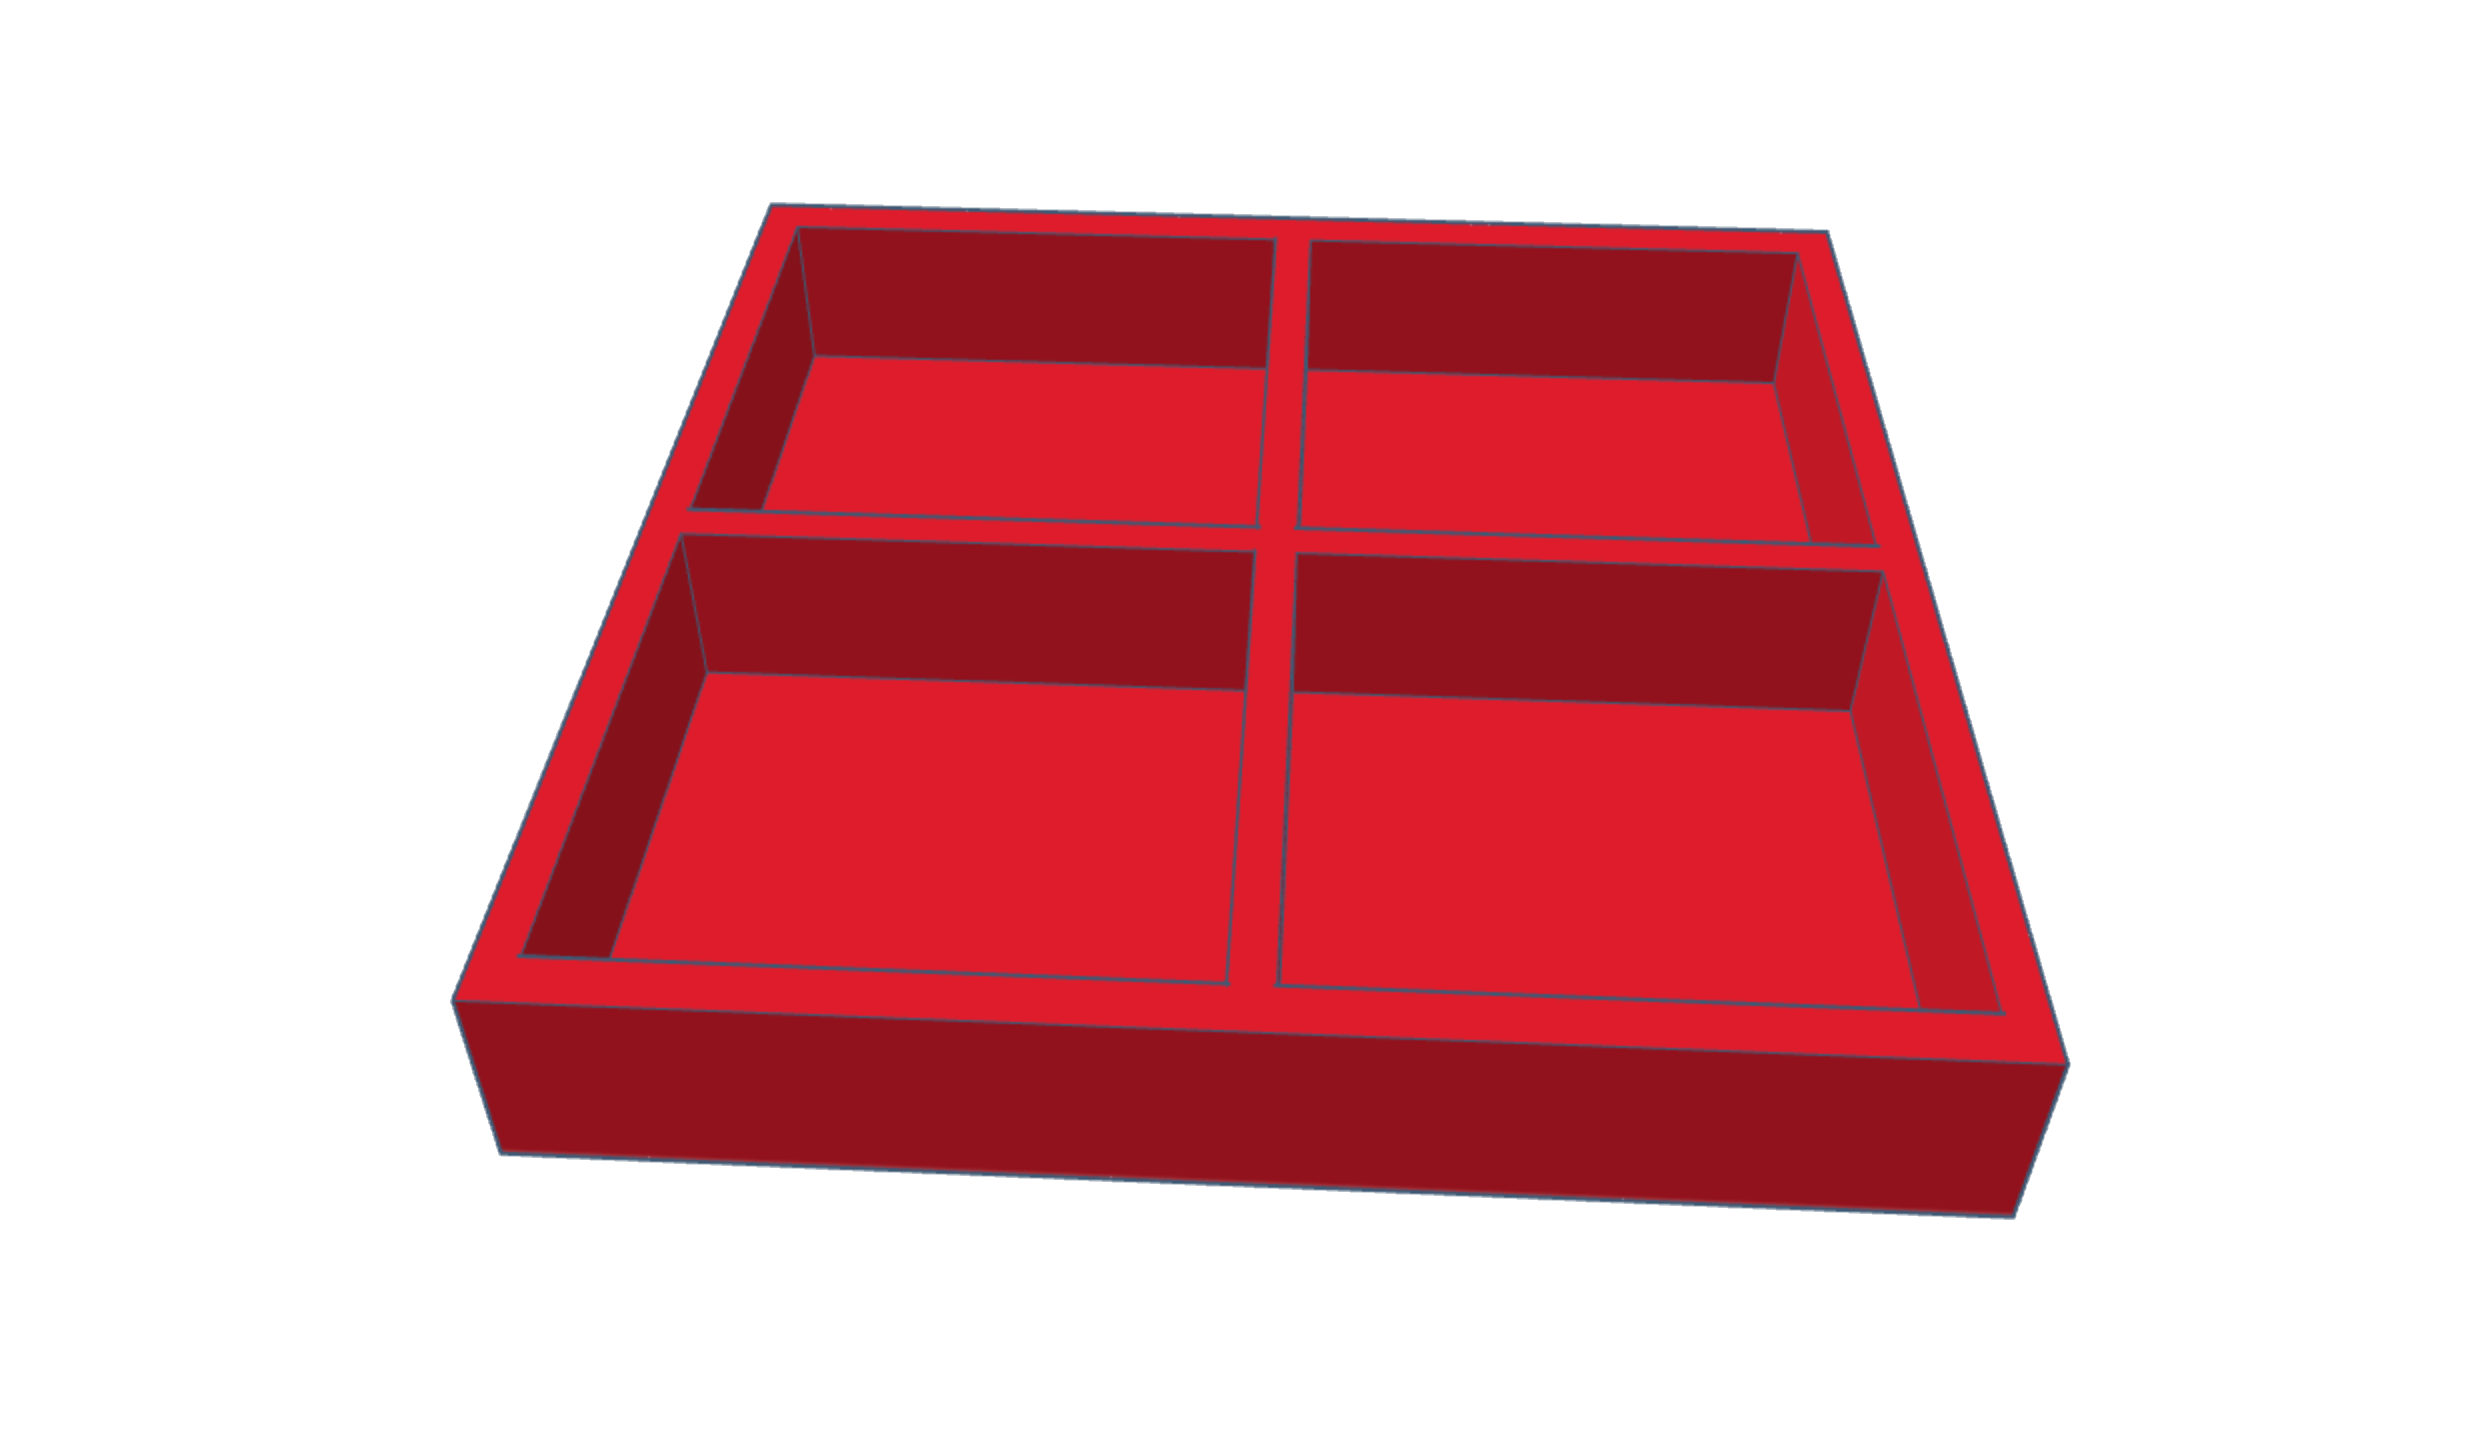
\includegraphics[width=\linewidth]{secciones//images/cajon3D.png}
        \caption{Diseño 3D}
    \end{subfigure}
    \hfill
    \begin{subfigure}[b]{0.45\linewidth}
        \centering
        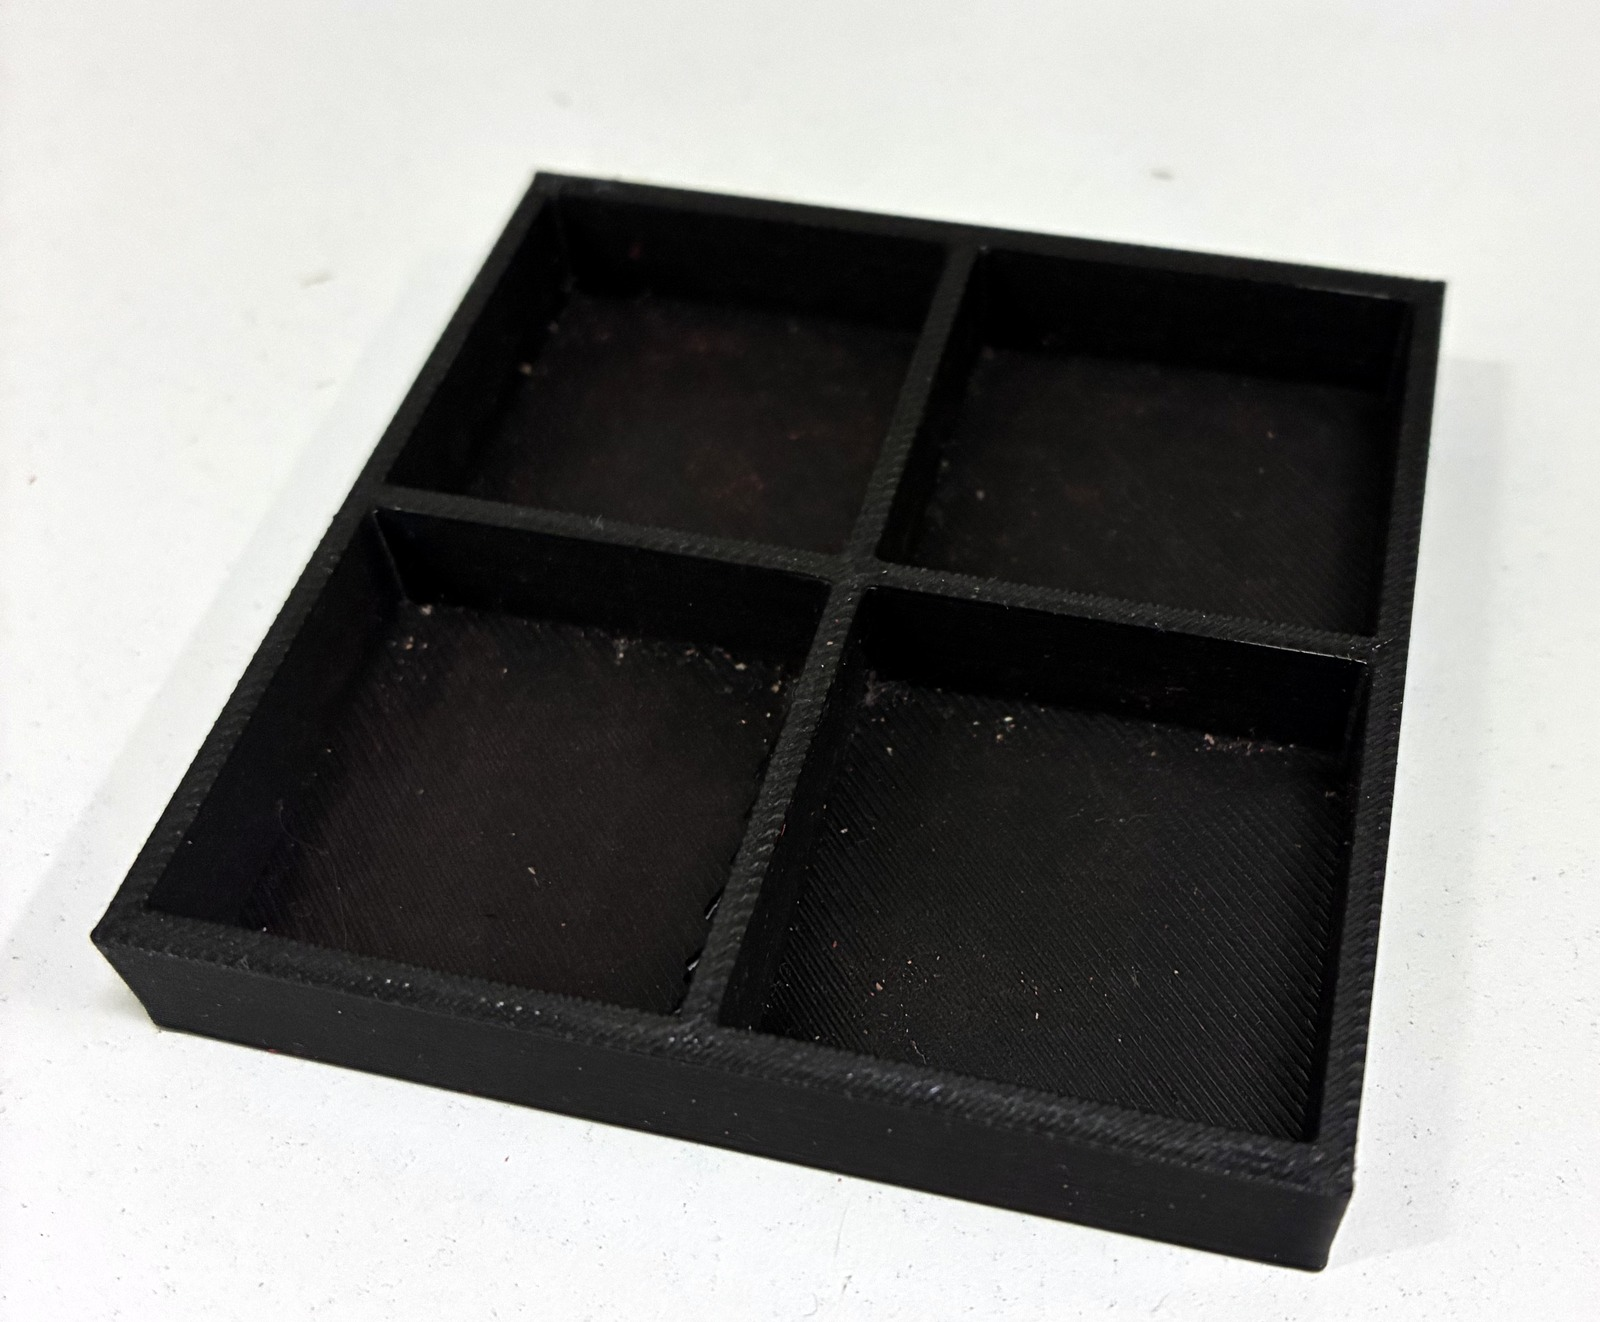
\includegraphics[width=\linewidth]{datos/img/cajon_foto.jpg}
        \caption{Pieza impresa}
    \end{subfigure}
    \caption{Cajón portasemillas con cuatro compartimentos para el alojamiento de semillas: diseño y pieza fabricada mediante impresión 3D.}
    \label{fig:cajon_semillas}
\end{figure}

\subsubsection{Piezas auxiliares para manipulación experimental}

Además de la estructura principal de tratamiento, se diseñaron piezas auxiliares destinadas a facilitar distintas etapas del trabajo experimental. Entre ellas se incluyó una cubierta parcial para cajones y una cuchara medidora para la dosificación de semillas.

\subsubsection{Dispositivo de dosificación de semillas}

Con el fin de evitar el conteo manual repetido de 20 semillas por muestra, se diseñó una cuchara medidora orientada a dosificar aproximadamente esa cantidad con la menor variabilidad posible. Dado que el volumen ocupado por las semillas depende de su tamaño y disposición, se optó por un diseño paramétrico utilizando \textit{build123d}, lo que permitió modificar de manera sistemática las dimensiones de la pieza.

A partir de un diseño inicial, se generaron variantes con cambios de tamaño del orden de $\pm 5\%$, con el objetivo de evaluar cuál de ellas se ajustaba mejor a una carga cercana a 20 semillas de maíz por uso. Las distintas versiones fueron fabricadas mediante impresión 3D y comparadas experimentalmente, seleccionándose finalmente aquella que mostró el mejor ajuste al valor buscado y una menor variabilidad entre repeticiones. La caracterización de la cuchara seleccionada, realizada a partir de 108 mediciones, mostró una media de 17,44 semillas por carga, una mediana de 17,00 semillas y una desviación estándar de 2,08 semillas. Se agradece a Lucía Guerreiro por la obtención y provisión de estos datos.

La Figura~\ref{fig:cuchara3D} muestra, lado a lado, el diseño digital y la cuchara medidora ya impresa. Los archivos de diseño correspondientes se encuentran documentados en el repositorio del proyecto.

\begin{figure}[H]
    \centering
    \begin{subfigure}[b]{0.45\linewidth}
        \centering
        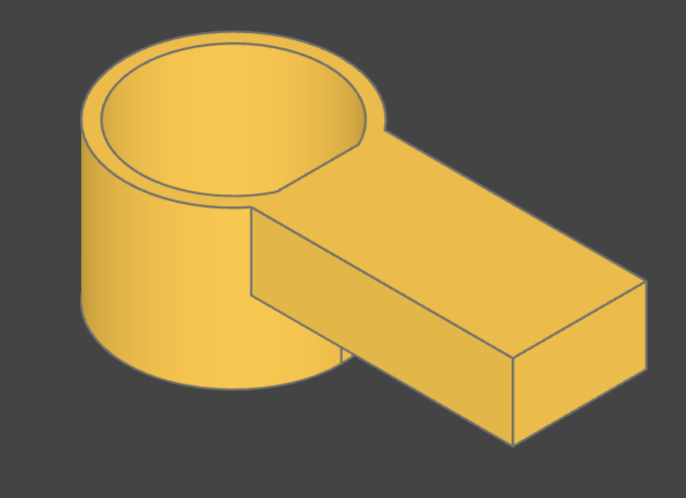
\includegraphics[width=\linewidth]{secciones//images/cuchara3D.png}
        \caption{Diseño 3D}
    \end{subfigure}
    \hfill
    \begin{subfigure}[b]{0.45\linewidth}
        \centering
        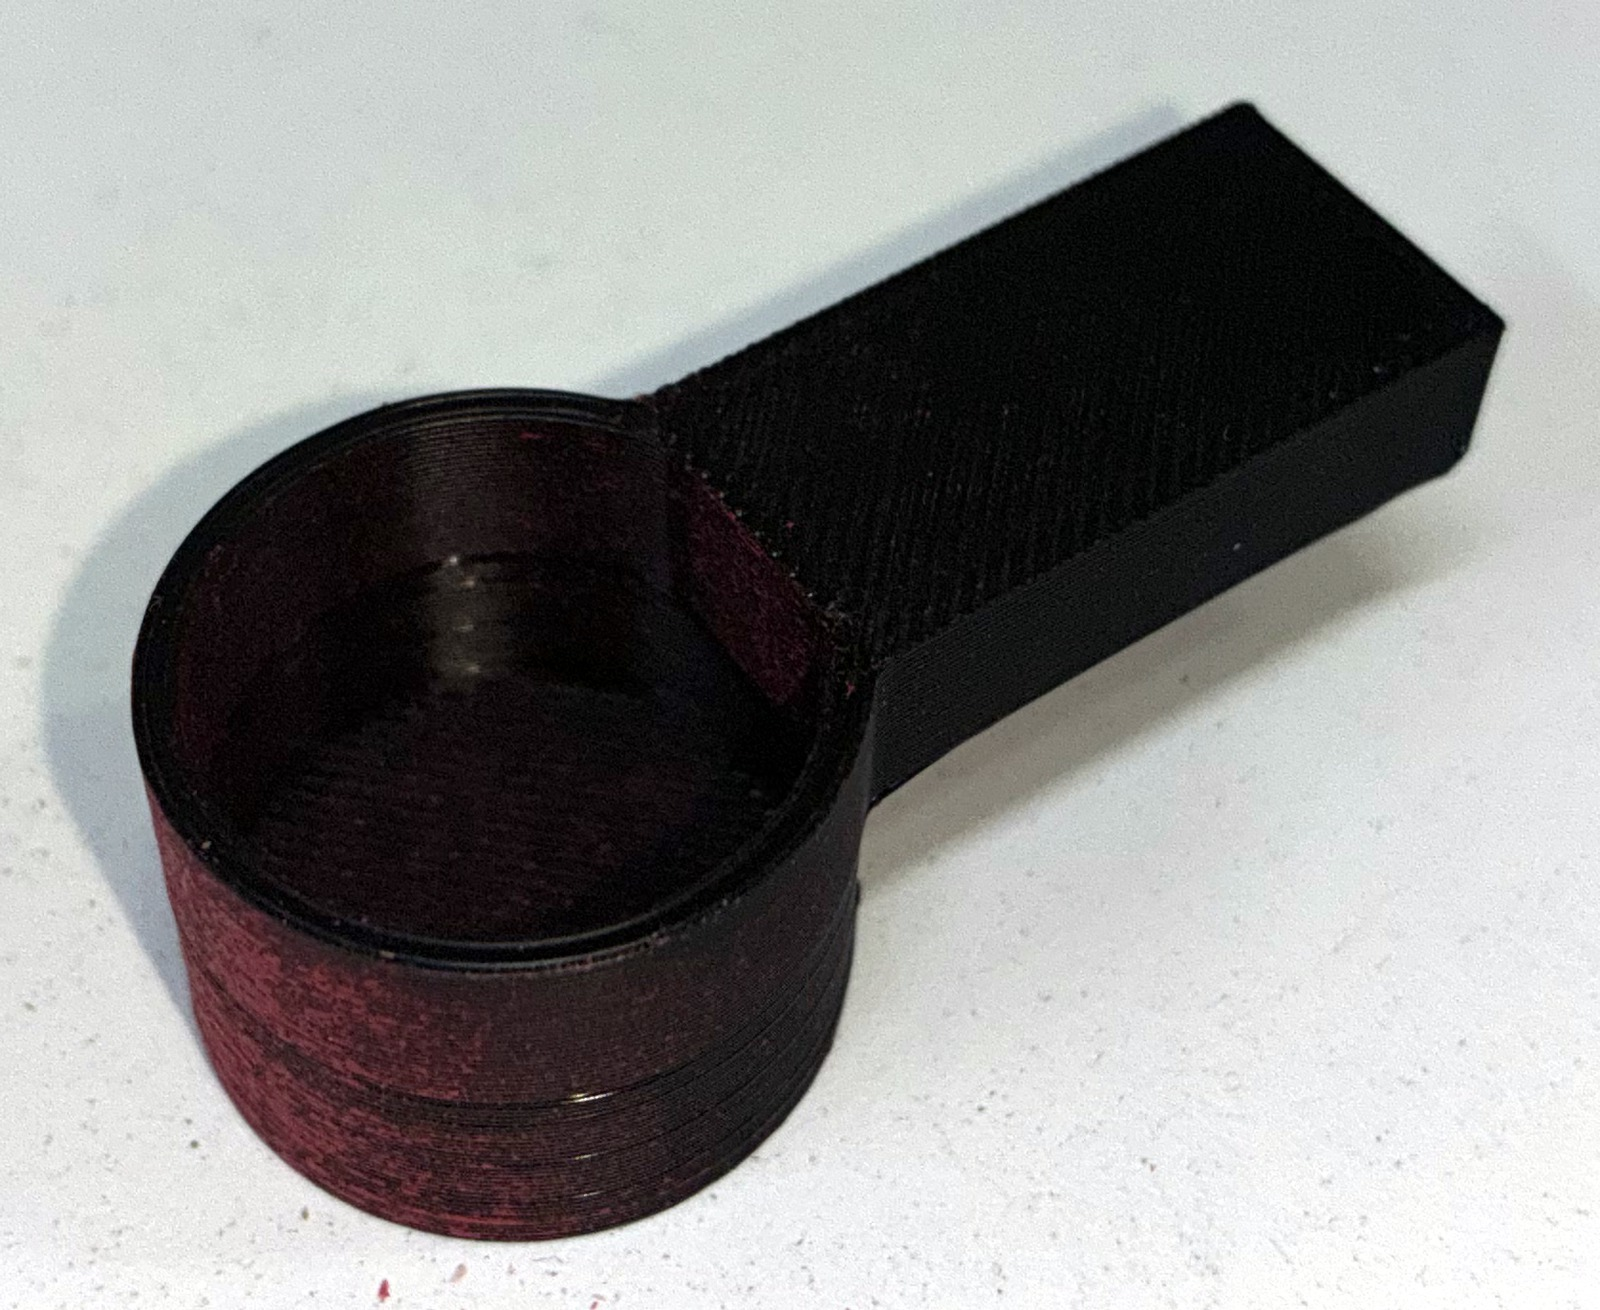
\includegraphics[width=\linewidth]{datos/img/cuchara_foto.jpg}
        \caption{Pieza impresa}
    \end{subfigure}
    \caption{Cuchara medidora desarrollada para dosificar aproximadamente 20 semillas de maíz: diseño y pieza fabricada mediante impresión 3D.}
    \label{fig:cuchara3D}
\end{figure}

\begin{figure}[H]
    \centering
    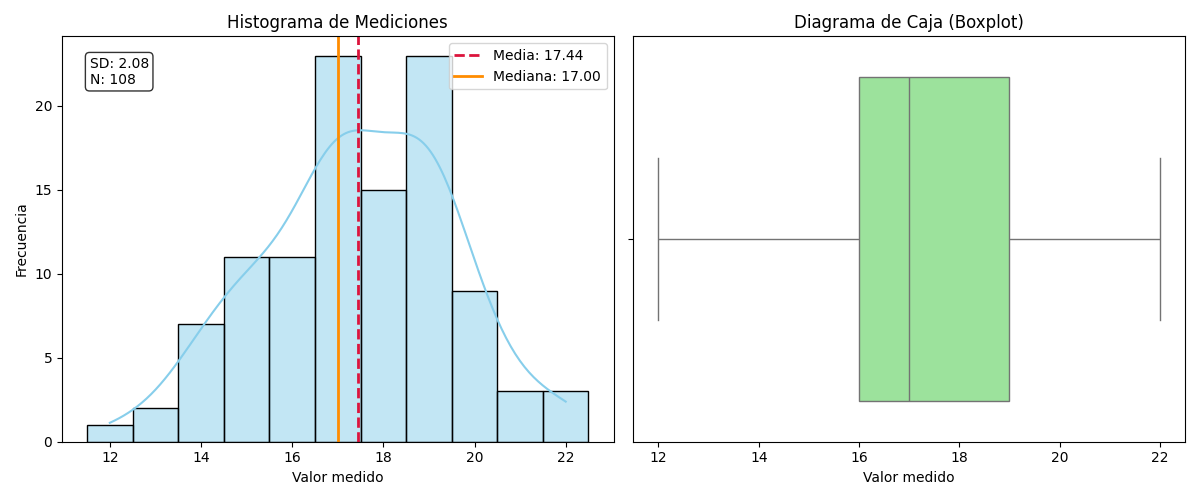
\includegraphics[width=\linewidth]{secciones//images/CaracterizacionCucharaPlots.png}
    \caption{Caracterización experimental de la cuchara medidora seleccionada. Se muestra la distribución de las mediciones de cantidad de semillas por carga y el diagrama de caja correspondiente.}
    \label{fig:caracterizacion_cuchara}
\end{figure}

\subsubsection{Construcción del photobox}

Para la adquisición de imágenes de semillas germinadas se construyó un \textit{photobox}, consistente en una caja con fondo negro e iluminación LED. Este dispositivo fue diseñado con el propósito de mejorar el contraste de las imágenes y estandarizar las condiciones de captura, reduciendo la variabilidad asociada a la iluminación y al fondo durante la toma fotográfica.

La utilización de este sistema permitió obtener imágenes en condiciones más homogéneas, facilitando posteriormente el procesamiento automático de las radículas mediante software.

\subsection{Procedimiento experimental}

Los experimentos se llevaron a cabo empleando el sistema de torre, semilleros y cajones diseñado para este trabajo. Las semillas fueron distribuidas en bandejas o recipientes identificados de forma individual, de manera de conservar la trazabilidad de cada unidad experimental durante las distintas etapas del protocolo.

La organización espacial de las muestras dentro del sistema experimental fue asistida mediante una asignación controlada de posiciones, con el objetivo de ordenar la disposición de las semillas dentro del montaje y disminuir posibles sesgos asociados a la ubicación de las muestras. Asimismo, se procuró mantener condiciones de trabajo reproducibles durante las etapas de preparación, tratamiento, germinación y registro.

Luego del tratamiento y de la etapa de germinación, las muestras fueron fotografiadas utilizando el \textit{photobox} construido para este trabajo. Dichas imágenes constituyeron la base para el procesamiento posterior de las radículas mediante herramientas computacionales específicas.

\subsection{Registro de datos}

Con el fin de asegurar un registro sistemático de la información experimental, se generó para cada ensayo una estructura de directorios y archivos en la que se almacenaron tanto los datos descriptivos del experimento como los resultados obtenidos durante las distintas etapas del trabajo.

En particular, se registró la identificación de cada bandeja, su posición dentro del montaje experimental, la asignación correspondiente dentro del esquema de tratamiento y metadatos asociados al experimento, tales como el imán utilizado y el polo enfrentado a las semillas. Asimismo, se incorporó la posibilidad de registrar pesos iniciales y finales de cada unidad experimental, facilitando una organización estructurada de la información.

Las fotografías adquiridas durante la etapa de germinación también fueron almacenadas de manera ordenada dentro de la estructura del proyecto, de modo de conservar la trazabilidad entre las imágenes, las bandejas y los resultados del análisis posterior.

\subsection{Herramientas computacionales desarrolladas}

Además del desarrollo del montaje físico, se implementaron herramientas computacionales orientadas a asistir la organización del experimento, el registro de datos y el procesamiento automático de imágenes. Estas herramientas constituyeron un soporte metodológico para mejorar la trazabilidad, reproducibilidad y eficiencia del flujo de trabajo experimental.

\subsubsection{Asignador de bandejas}

Como parte de las herramientas computacionales desarrolladas para este trabajo, se implementó un programa en Python destinado a la asignación y gestión de las bandejas experimentales. Su propósito fue asistir la organización de cada ensayo mediante la creación automática de la estructura de archivos asociada al experimento, la generación del archivo \texttt{trays.csv} y la asignación aleatoria de los tratamientos a las posiciones físicas disponibles en el arreglo experimental.

El programa permitió definir e identificar cada bandeja de manera unívoca, asociándola al experimento correspondiente y a su posición dentro del montaje. Además, incorporó el registro de metadatos experimentales, tales como el imán utilizado y el polo enfrentado a las semillas. De este modo, se facilitó la trazabilidad de cada unidad experimental y la conservación ordenada de la información relevante para el posterior análisis de datos.

Adicionalmente, la herramienta incluyó una interfaz para la carga y actualización de los pesos iniciales y finales de las bandejas, con sugerencias automáticas de la siguiente posición a completar. Esta funcionalidad permitió agilizar la carga secuencial de datos y reducir la probabilidad de errores manuales durante el registro. En conjunto, el asignador de bandejas constituyó una herramienta auxiliar para estandarizar la organización del experimento, mejorar la reproducibilidad del procedimiento y favorecer la consistencia del registro experimental.

En la Figura~\ref{fig:asignador-bandejas} se muestra una captura de la interfaz gráfica desarrollada para esta herramienta.

\begin{figure}[H]
    \centering
    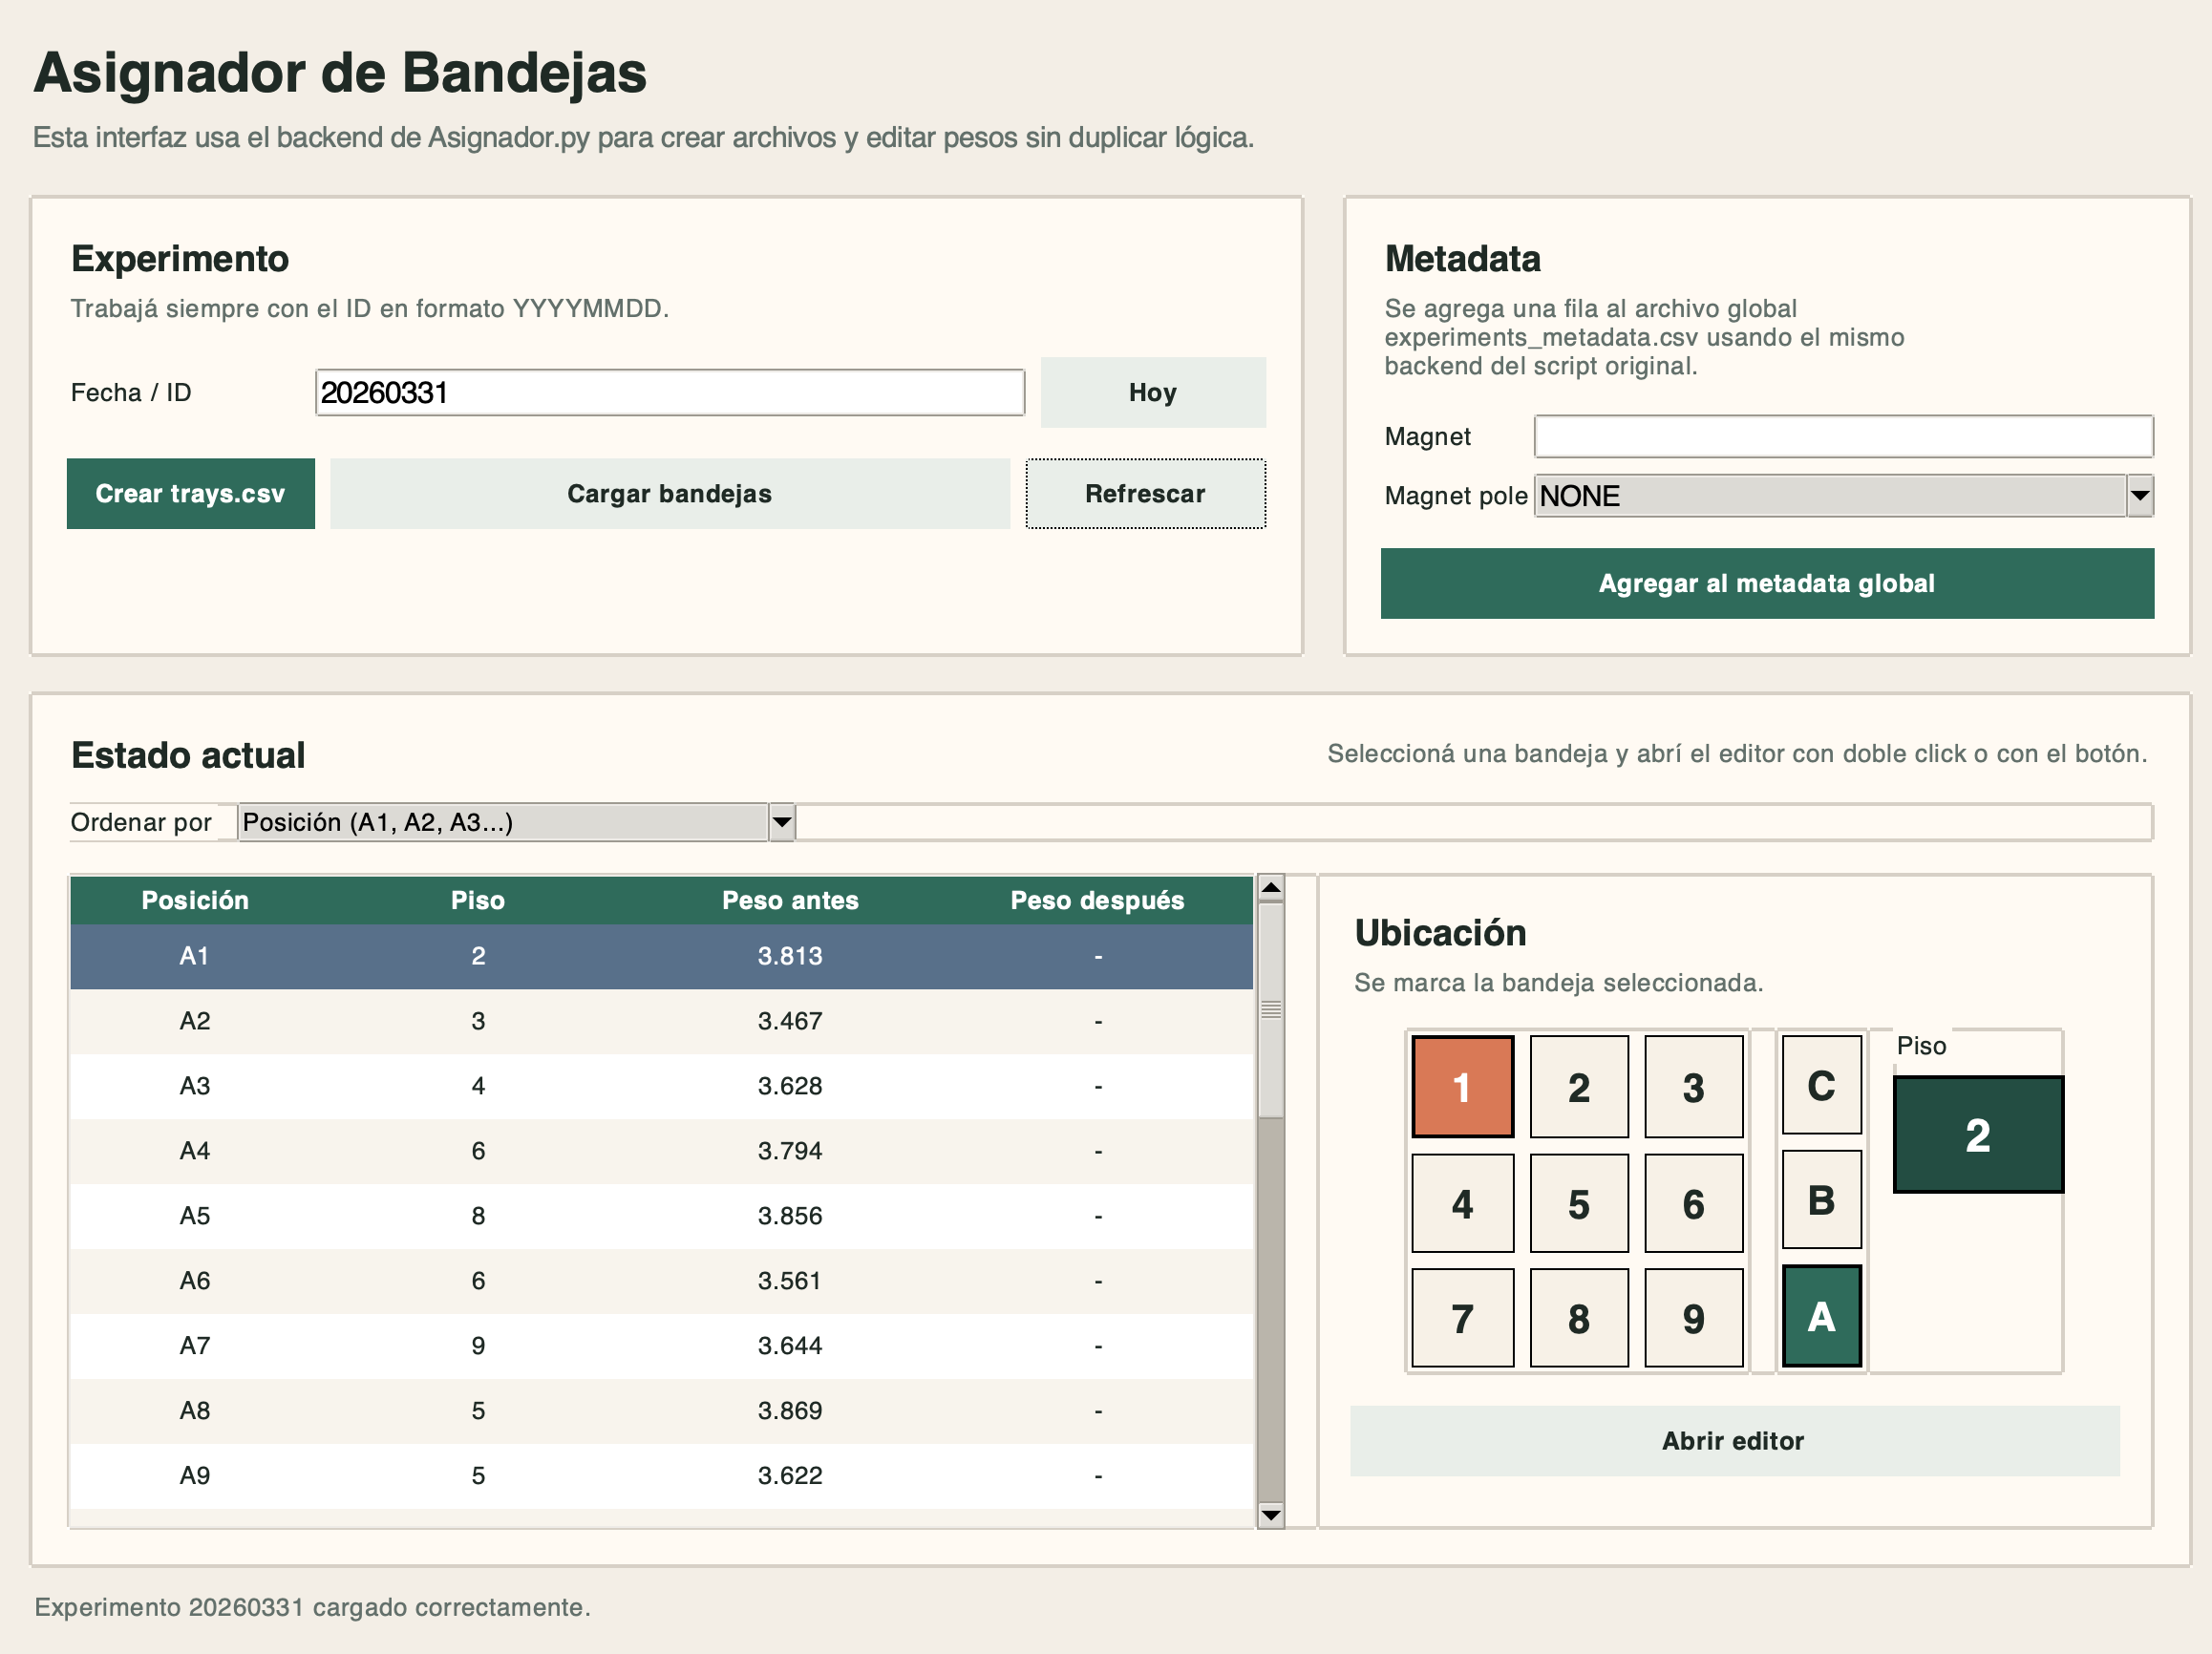
\includegraphics[width=0.75\linewidth]{secciones//images/asignadorGUI.png}
    \caption{Interfaz gráfica del programa desarrollado para la asignación y gestión de bandejas experimentales.}
    \label{fig:asignador-bandejas}
\end{figure}

\subsection{Procesamiento y análisis de datos}

Una vez adquiridas las imágenes de las semillas germinadas, se realizó un procesamiento automático orientado a extraer parámetros cuantitativos asociados al crecimiento de las radículas. Para ello se desarrolló una herramienta específica que permitió identificar estructuras de interés en las imágenes, medir sus longitudes y almacenar los resultados obtenidos de manera organizada para su posterior análisis.

\subsubsection{Software de detección y medición de radículas}

Se desarrolló una herramienta de software para el procesamiento automático de imágenes de semillas germinadas, con el objetivo de estimar la longitud de las radículas a partir de fotografías adquiridas mediante el \textit{photobox}. El programa permite identificar las radículas presentes en cada imagen, calcular sus longitudes individuales y obtener medidas agregadas, como la longitud media de radícula por muestra.

La implementación de esta herramienta tuvo como finalidad reducir la intervención manual en la etapa de medición, mejorar la reproducibilidad del procesamiento y facilitar el almacenamiento sistemático de los resultados experimentales. Los datos generados por el software fueron utilizados posteriormente en la etapa de análisis.

La Figura~\ref{fig:software_radiculas} presenta una captura de pantalla de la interfaz o entorno de uso del software desarrollado. El código correspondiente se encuentra disponible en el repositorio del proyecto.

\begin{figure}[H]
    \centering
    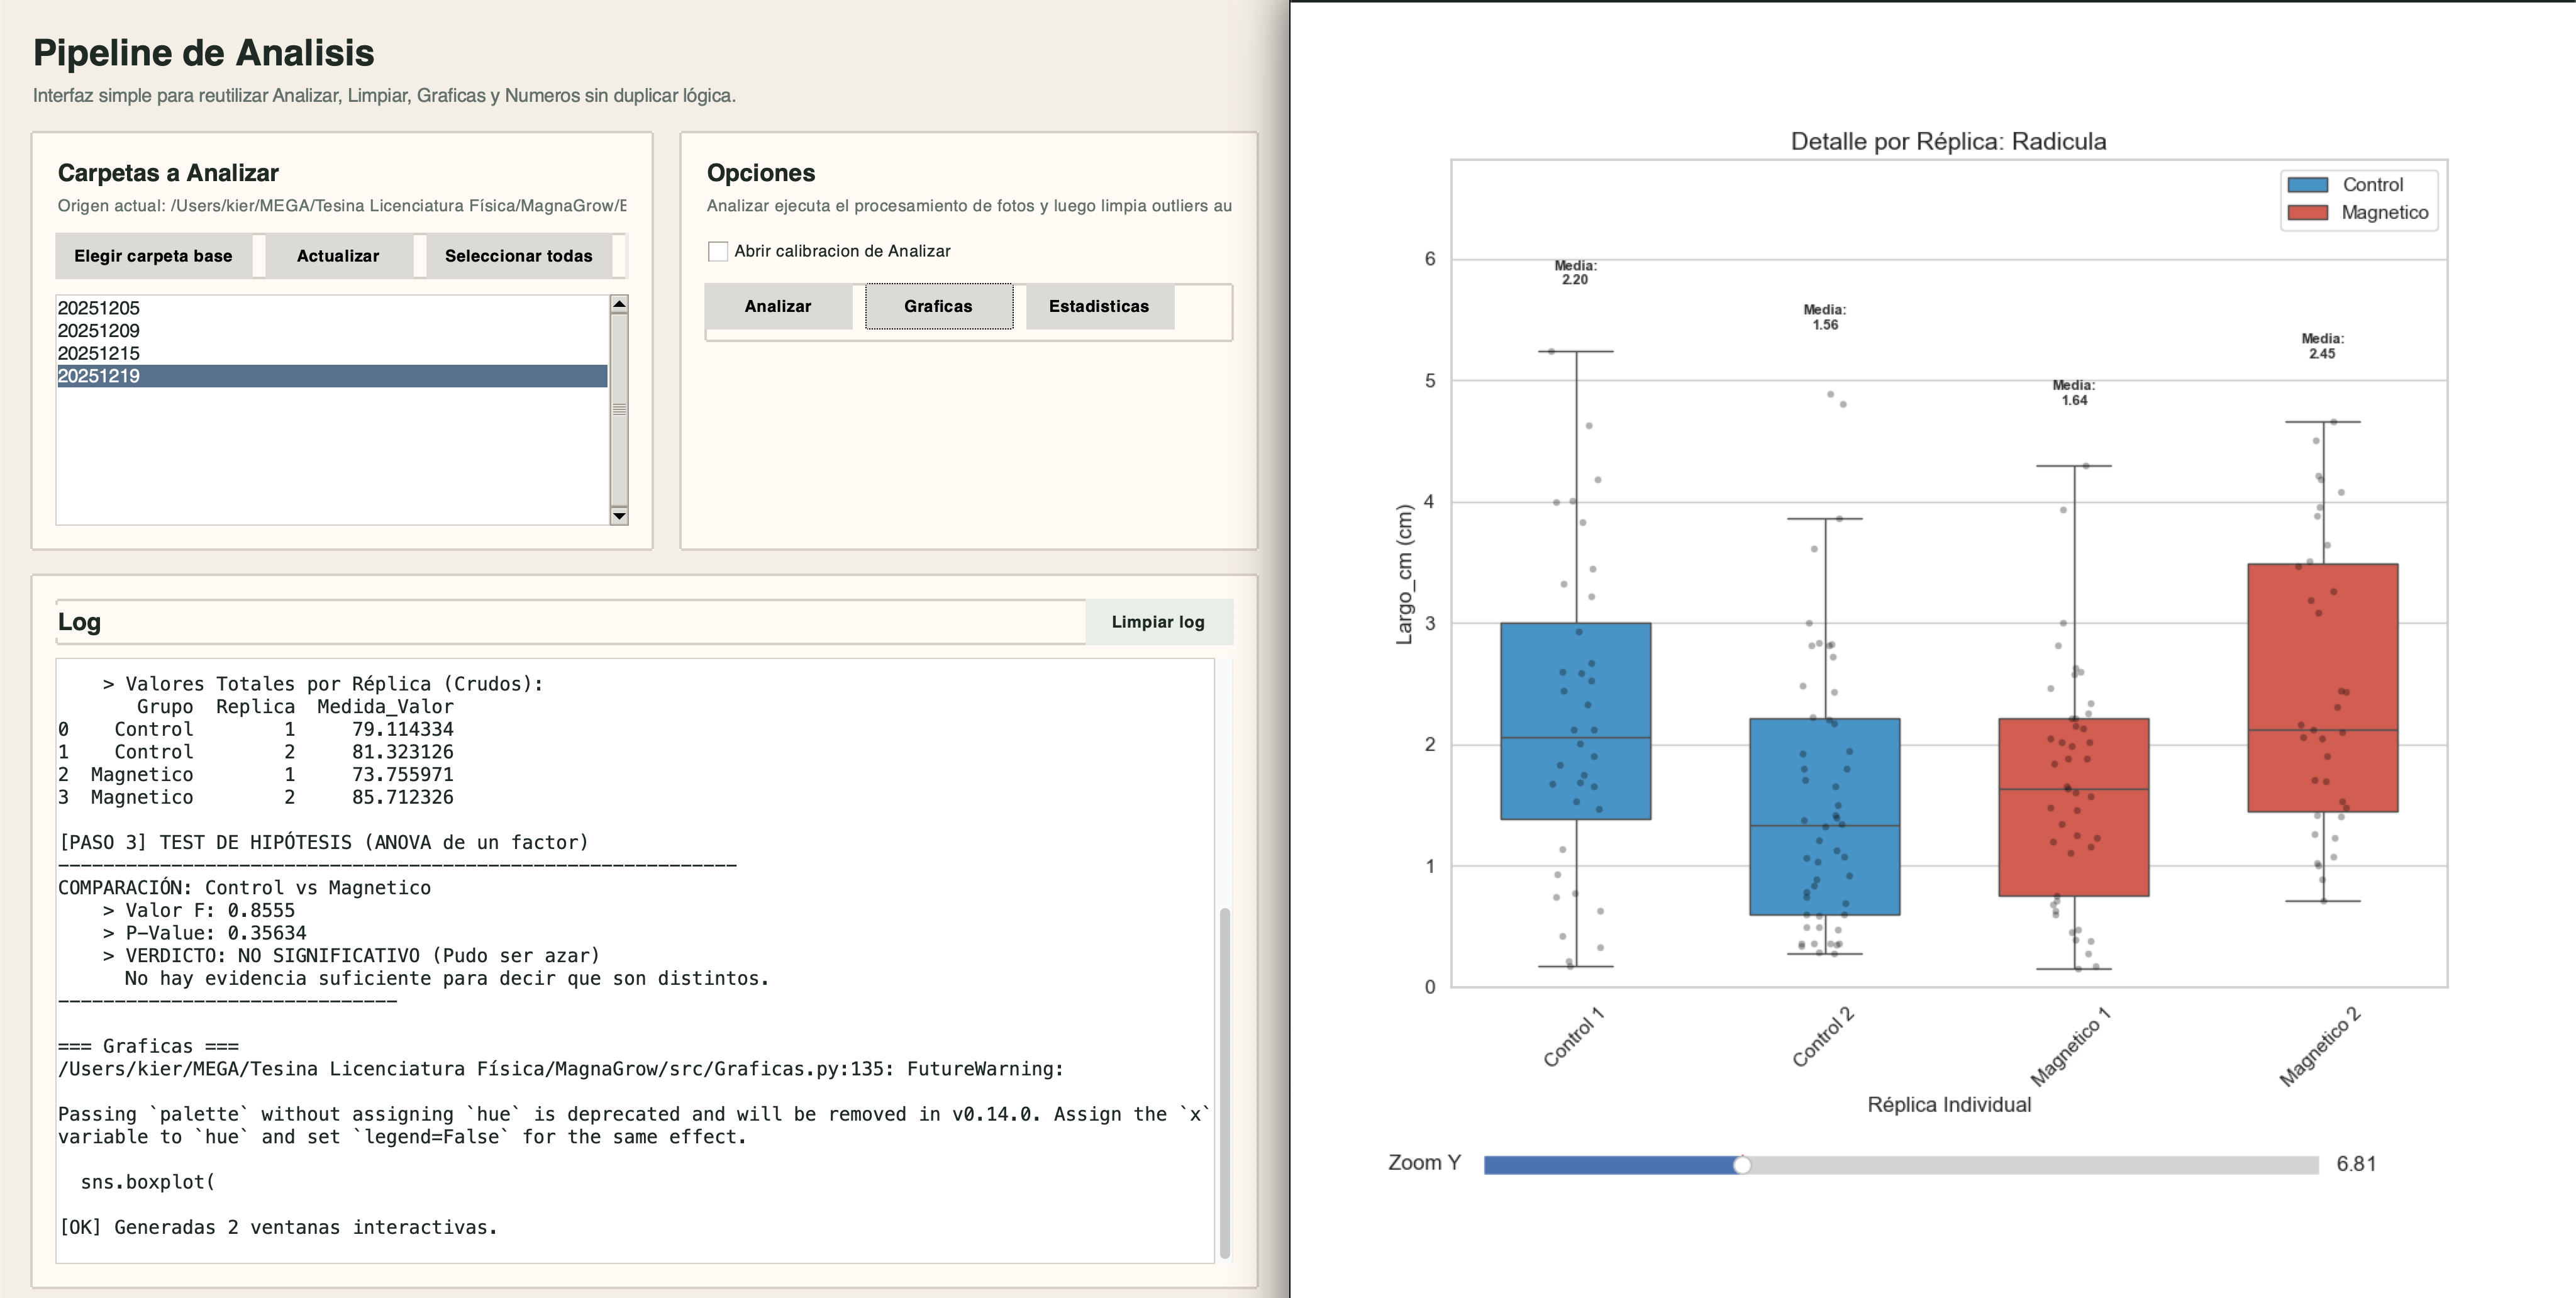
\includegraphics[width=1\linewidth]{secciones//images/pipelineGUI.png}
    \caption{Interfaz del software desarrollado para el procesamiento de imágenes y la obtención de parámetros cuantitativos a partir de fotografías de semillas germinadas.}
    \label{fig:software_radiculas}
\end{figure}

\subsection{Experimentos control negativo}

Con el objetivo de caracterizar la variabilidad basal del sistema experimental y establecer una línea de referencia para la comparación con los tratamientos magnéticos, se realizaron tres experimentos control independientes en los que las semillas no estuvieron expuestas a ningún campo magnético. Estos experimentos se llevaron a cabo en las fechas 04/04/2026, 28/04/2026 y 07/05/2026.

Cada experimento control consistió en 27 bandejas experimentales, distribuidas en 3 pisos (A, B, C) y 9 posiciones, siguiendo la misma disposición geométrica y el mismo protocolo de germinación, registro fotográfico y procesamiento de imágenes que los experimentos con tratamiento. No se colocaron imanes en ninguna de las bandejas durante la etapa de exposición.

El diseño repetido en el tiempo permitió evaluar la reproducibilidad del protocolo y cuantificar la variabilidad interexperimento atribuible a factores no controlados, como fluctuaciones ambientales o diferencias entre lotes de semillas. Asimismo, el diseño espacial (piso y posición) posibilitó la detección de posibles sesgos sistemáticos dentro del montaje experimental, información relevante para la interpretación de los resultados de los experimentos con tratamiento.
